\documentclass[11pt,a4paper,oneside]{article}
\usepackage[utf8]{inputenc}
\usepackage{amsmath}
\usepackage{amsfonts}
\usepackage{amssymb}
\usepackage{graphicx}
\usepackage{geometry}
 \geometry{
 a4paper,
 total={170mm,257mm},
 left=20mm,
 top=20mm,
 }
\author{John Walmsley, Gary R. Mirams}
\title{Predicting simulation-experiment discrepancy in cell-specific cardiac electrophysiology models}

\newcommand{\norm}[1]{\left\lVert#1\right\rVert}

\begin{document}

\maketitle

\section{Introduction}


\section{Models of the hERG Channel} \label{}


\section{Definition of Discrepancy} \label{ModelsOfDiscrepancy}
\subsection{Simulation discrepancy}
"Model discrepancy" can be defined in different ways. For the purposes of this project, we will be using two different definitions. The first (in line with the CIPA goals described above) is the discrepancy between the model and the target trace $I_{exp}$, which may be experimental data or some other simulated data. We can sub-divide this definition in terms of how we consider this discrepancy. The first method is very simple:
\begin{align}
	I_{exp} = G O ( V - V_E ) + d\\
	d = I_{exp} - G O ( V - V_E )
\end{align}
This is the difference between model simulation and data, used in \cite{Beattie2018} in the least squares fitting procedure. The second definition is more natural from a physiological point of view, but less well behaved mathematically. Because the measured current is proportion to the open probability of the channel and the (known) voltage, we can also consider
\begin{align}
	I_{exp} = G ( O + d_o ) ( V - V_E )\\
	d_o = \frac{I_{exp} }{ G( V - V_E ) } - O
\end{align}
Because of the singularity around the Nernst potential $V_E$, we need to remove these points from the trace - most traces spend relatively little time at these potentials (\~-88mV). In this project, a 5mV window either side of the Nernst potential was discarded. These definitions of discrepancy are used in Sections \ref{SubSec_Lasso_Discrepancy} and \ref{SubSec_StepwiseLM_Discrepancy}. Plots of both forms of discrepancy for the sine wave and action potential protocols are shown in Fig.~\ref{Fig_Discrepancy}.

\begin{figure}[t]
\begin{center}
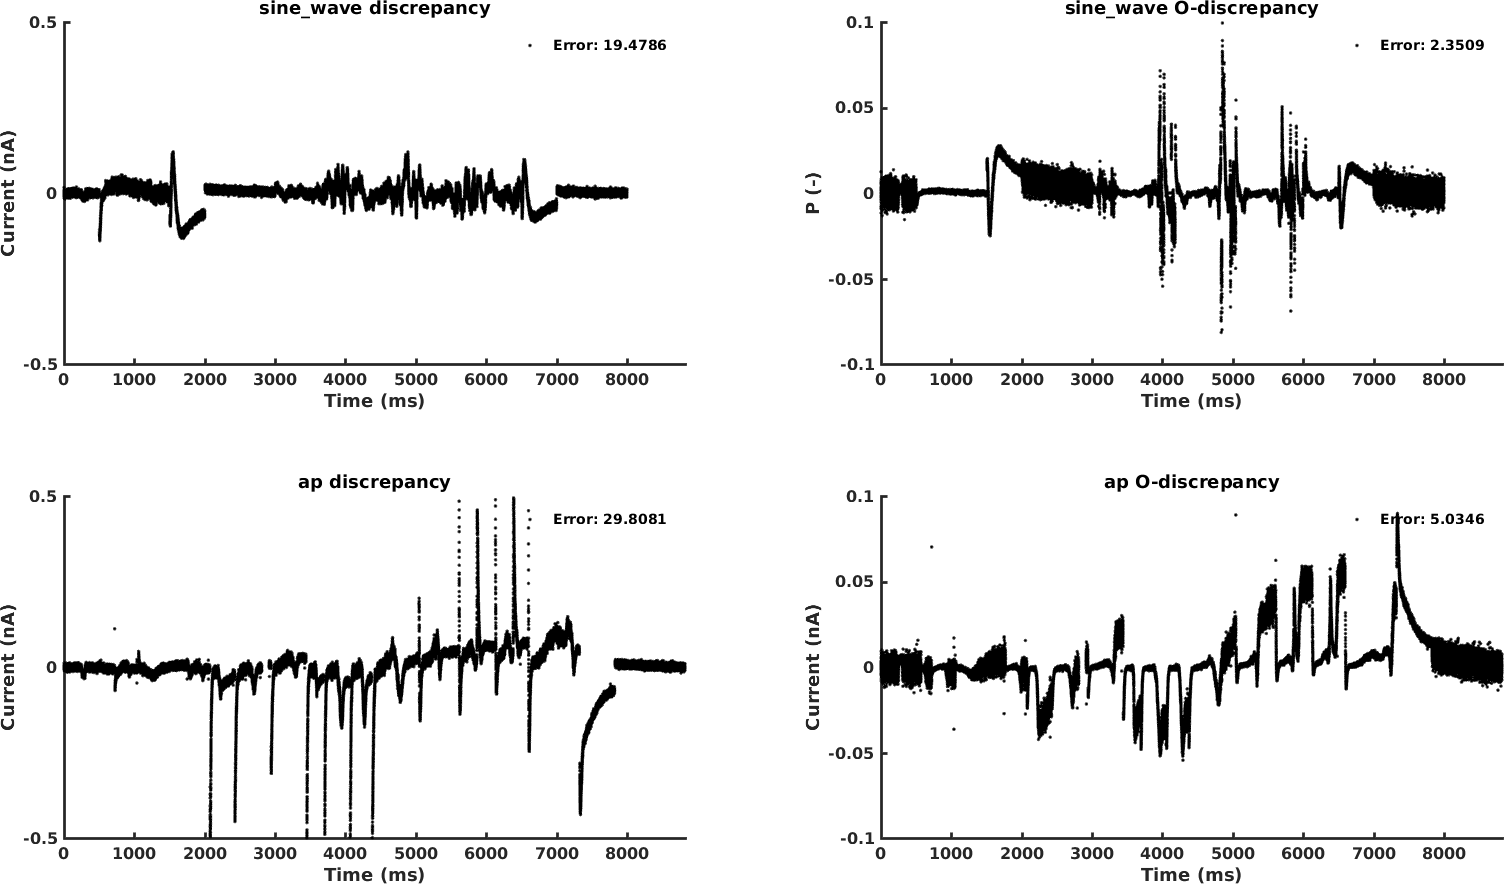
\includegraphics[scale=0.42]{Figures/PlotDiscrepancyVsDiscrepancyInOpen_sine_wave_ap.png}
\caption{\textbf{Discrepancies for the sine wave (top) and action potential (bottom) protocols.} The left hand column shows $d$ and the right hand column shows $d_o$. Capacitative spikes have been removed.}
\label{Fig_Discrepancy}
\end{center}
\end{figure}


\subsection{Structural discrepancy}
Both of the above definitions rely on a particular parameterisation of the model. However, it is also possible to consider the model discrepancy as being the difference between the model and reality. This concept is explained in more detail in \cite{Kennedy2001} and \cite{Strong2014} and refers to the structure of the model rather than its parameterisation.  This definition of model discrepancy refers to model structure, rather than model parameterization (which would change $d$ and $d_o$, above). In the context of hERG modelling, this could be a relatively simple difference, such as the number of closed states in a model or the form of the rate constants. Alternatively, it could be an entirely different feature not preserved in the model of interest - consider the difference between a molecular dynamics simulation of channel opening and a four state Markov model. In this project, we considered this form of discrepancy by fitting four models to the same data and then exploring how their evolution differed in time (Section \ref{}).

\section{Statistical Prediction of Discrepancy}

\subsection{Introduction}

Our goal was to predict simulation discrepancy when using fitted models for prediction. The goal would then be to quantify, based on the training data and the prediction simulation, where and by how much the prediction simulation would differ from the actual experimental trace recorded from that cell, for the prediction protocol. In this report, we use two methods, LASSO and the Matlab method Stepwise Linear Model.

\subsection{Input Variables}

As an initial hypothesis, we proposed to use properties derivable from the model equations shown in Eqs. \eqref{}-\eqref{}. These properties are
\begin{itemize}
\item Variables $y_1$, $y_2$, $y_3$, $y_4$.
\item Rates $K_{ij}$
\item Fluxes $y_i K_{ij}$
\item Current $I$
\item Voltage $V$
\item Voltage time derivative $\frac{dV}{dt}$
\item Time $t$
\item Parameter sensitivities $\frac{dy_i}{dp_j}$
\item Current sensitivity $\frac{dI}{dp_j} = G \frac{dy_3}{dp_j} (V-V_E) $
\end{itemize}

Parameter sensitivities are derived using the following equation \cite{}. Using $s_{ij} = \frac{dy_i}{dp_j}$,
\begin{align}
	\frac{\partial}{\partial p_j} ( \frac{dy_i}{dt} ) & = \frac{\partial}{\partial p_j} (f( y ) ) \\
	\frac{d}{dt}(\frac{\partial y_i}{\partial p_j})   & = \frac{\partial f}{ \partial y_i}\frac{\partial y_i}{ \partial p_j} + \frac{\partial f}{ \partial p_j} \\
	\frac{d s_{ij}}{dt} & = \frac{\partial f}{ \partial y_i} s_{ij} + \frac{\partial f}{ \partial p_j}
\end{align}
The CVODES libraries are used to integrate the parameter sensitivity equations alongside the ODEs in Eqns \eqref{}-\eqref{}.

Before performing any estimation, we check for linear dependence of each set of properties in turn, then check for linear dependence of all the properties that remain. The linear independence check is numerical and performed using the Mathworks File Exchange program getLinearDependent.m. Note that we did not include the derivatives of the variables ($\frac{dy_i}{dt}$ because they are linear combinations of the fluxes.

\subsection{Experimental Data}
For the purposes of this study we restricted ourselves to one cell from the study by \cite{}, the `middle' cell in terms of quality that is used in most of the plots in that paper. This is cell number 16713110. A number of experimental voltage protocols are used in this study. The main focus is on the `sine wave' (SW) and `action potential' (AP) protocols used by Beattie \textit{et al}\cite{Beattie2018}. However, we also used some other protocols recorded during data collection for this study, namely the `Original Sine Wave' (OSW), `Equal Proportions' (EP), and `Mazahari-Wang Difference' (MWDD) protocols. All protocols used and the corresponding experimentally recorded current are shown in Fig.~\ref{Fig_Protocols}. For the purposes of fitting, all capacitance spikes were removed as in Beattie \textit{et al}\cite{Beattie2018}.

\begin{figure}[t]
\begin{center}
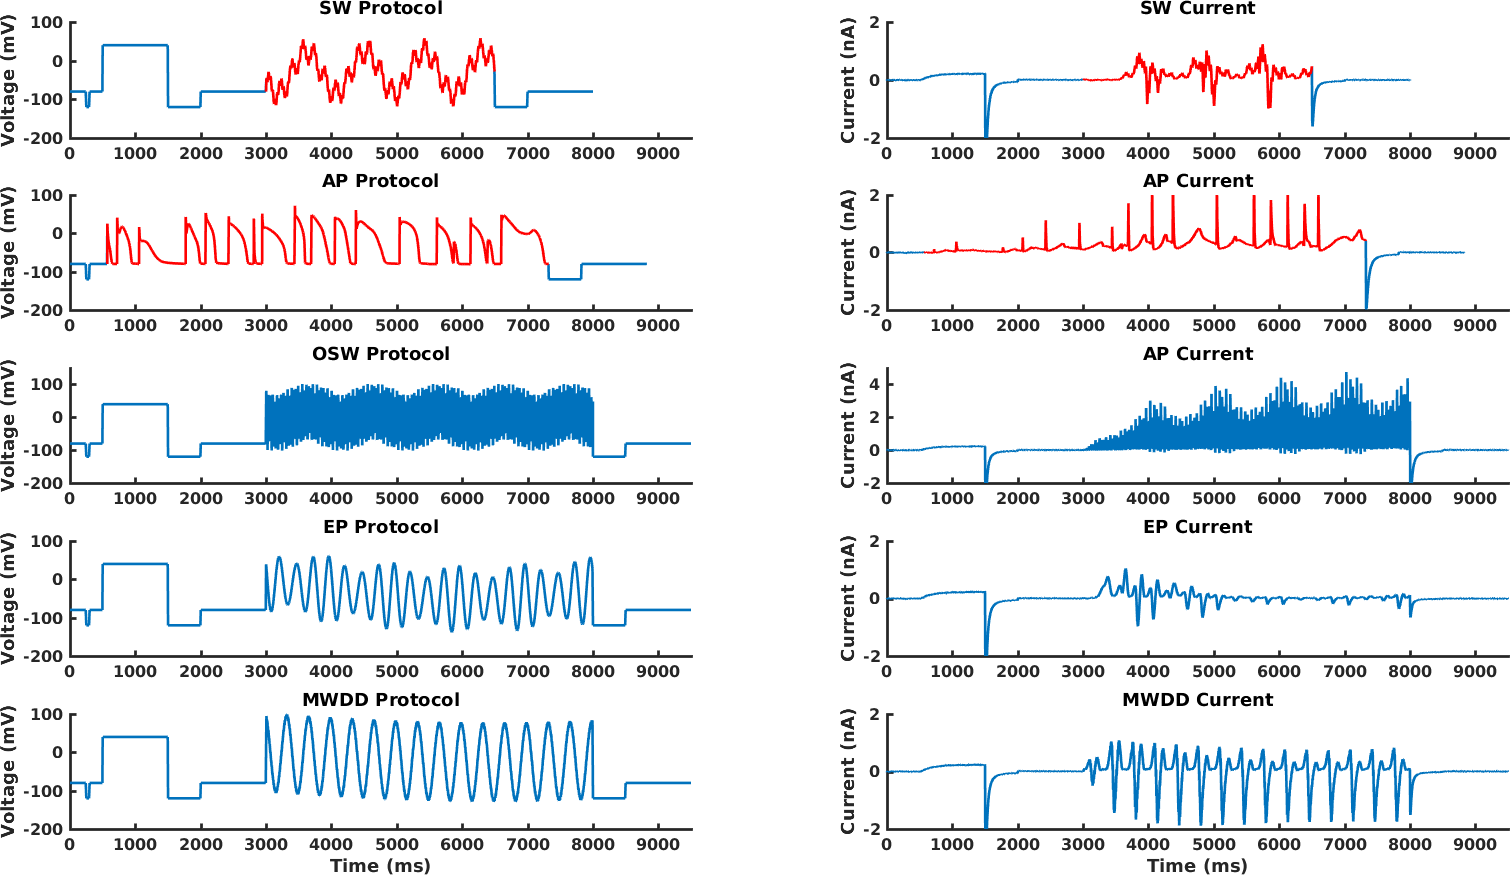
\includegraphics[scale=0.42]{Figures/Protocols.png}
\caption{\textbf{Protocols and current traces used in this report.} All five protocols and the resulting current traces for cell 16713110 as used in this study are shown with capacitative spikes removed. For the SW and AP protocols, the `core' of the protocol used in Sections \ref{SubSec_Lasso_Discrepancy} and \ref{SubSec_StepwiseLM_Discrepancy} are highlighted in red. Note that the y-axis scale for the OSW protocol and current differ from the other protocols due to the higher (and non-physiological) potentials reached - this was one reason for the rejection of the OSW protocol during the development of the SW protocol.}
\label{Fig_Protocols}
\end{center}
\end{figure}

\subsection{Predicting Discrepancy Using LASSO}\label{SubSec_Lasso_Discrepancy}

\subsubsection{The Method}
The Least Absolute Shrinkage and Selection Operator (LASSO) is a popular linear regression method that incorporates a regularization parameter $\lambda$. For a set of predictors $X$, $N$ data points $y$ and coefficients $\beta$, the LASSO method can be written in Lagrangian form as
\begin{align}
	\min_{\beta} ( \frac{1}{N} \norm{ y - \beta X }^2 + \lambda \norm{ \beta }^1 ).
\end{align}
The size of the parameter $\lambda$ determines the degree of regularization. Essentially, a large $\lambda$ penalizes $\beta$ heavily, and so produces smaller models. Conversely, a small $\lambda$ allows the method more freedom in the number of variables included. A key feature of the LASSO algorithm is that due to the $L_1$ norm used for regularization, elements of $\beta$ can be set to zero by the method, resulting in smaller models. This key property has made LASSO a popular method in Machine Learning. Variations on this method are Ridge regression (uses $\lambda \norm{ \beta }^2$ instead) and Elastic Net regression (a combination of Ridge and LASSO).

One challenge of the LASSO method is that there is no a priori choice for the regularization parameter $\lambda$. To determine $\lambda$ and check the validity of the resulting models we use K-fold cross-validation. This method works by splitting the experimental data into K equally sized folds, leaving one out, then checking the model's ability to predict the data in the left out fold. This results in an MSE for each fold, and for each value of $\lambda$. The variation in the MSE at each $lambda$ can be used to select $\lambda$ and hence, the model. To do so, we find the $\lambda$ value giving the minimum MSE, and then choose the largest $\lambda$ within one standard deviation from this point. This can be seen as choosing the smallest justifiable  model within the variation of the model that gives the absolute minium error. In this study, we use 10 folds which is a fairly standard choice.

An important property of K-fold cross-validation as inplemented in Matlab is that it uses random data points in each fold. While this is in principle a good thing, the extremely high time resolution of our data means that all of the resulting folds are likely to  be effectively the same, subject to experimental noise (see Fig.~\ref{}). As a result, the models produced by the Matlab algorithm were both non-predictive and non-deterministic. To correct for this, some editing of the Matlab source code is required (detailed in README.md). We instead split the trace into ten equal segments consecutive in time to ensure variation between folds.

\subsubsection{Results}

LASSO fits for a linear regression model of model discrepancy of $d$ and $d_o$ are shown in Figure \ref{Fig_LASSO_SW_AP_full_discrepancy}. For this model, the discrepancies resulting from the sine wave (SW) protocol developed in by Beattie et al.~was used as training data, and was used to predict the results from the action potential (AP) protocol used for validation in that study. The resulting corrected currents together with the original simulation and experimental data are shown in Fig.~\ref{Fig_LASSO_SW_AP_full_currents}. It can be appreciated that, in both cases, the linear models of discrepancy fail to predict the discrepancy observed in the AP trace.

\begin{figure}[t]
\begin{center}
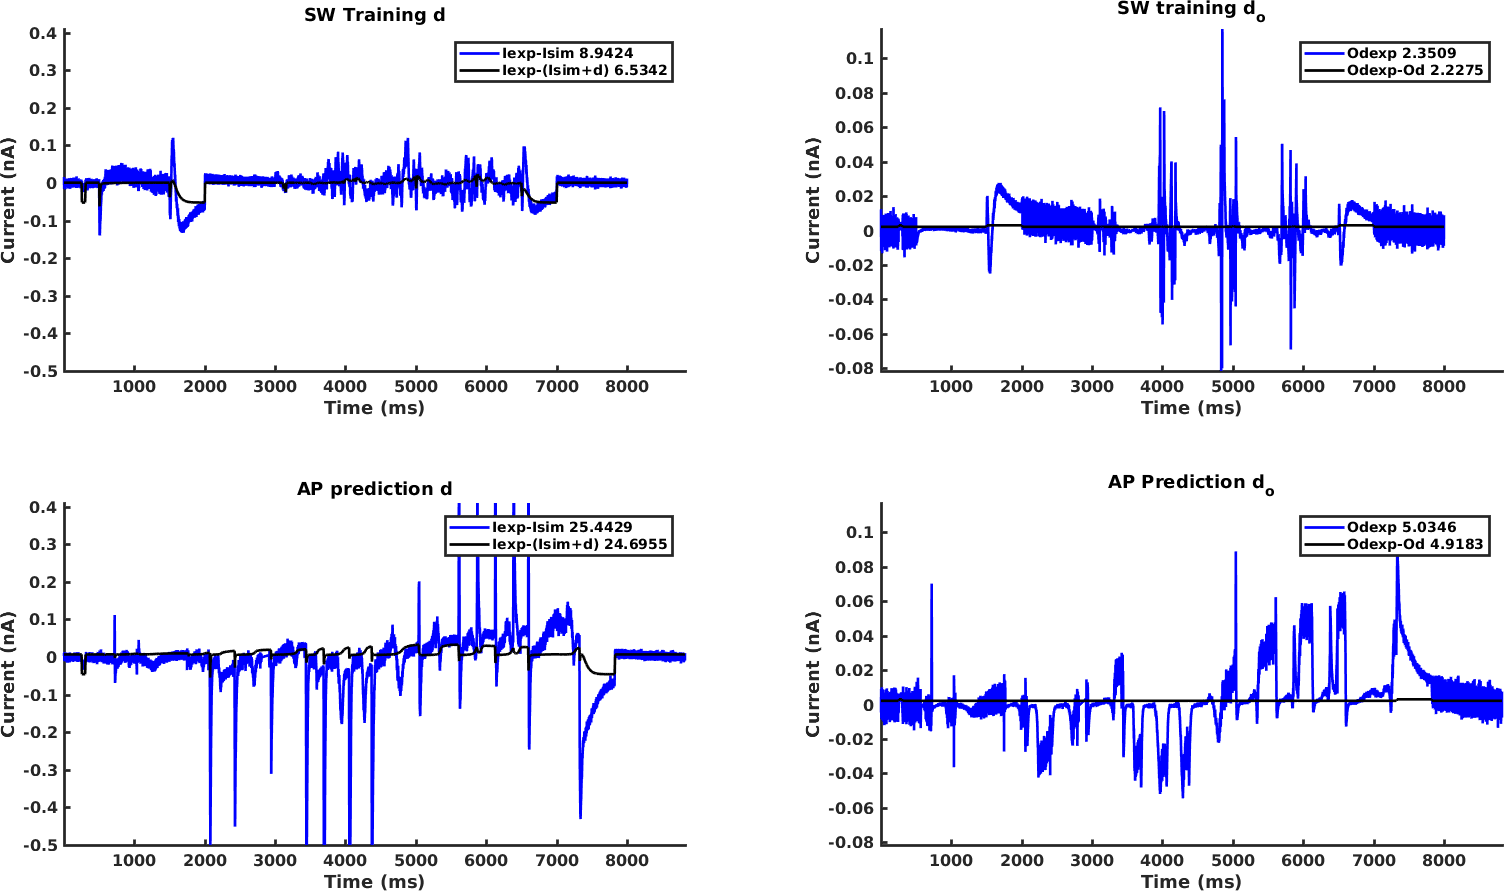
\includegraphics[scale=0.42]{Figures/LASSO_SW_AP_full_discrepancy.png}
\caption{\textbf{Linear model of discrepancy constructed using LASSO.} These models of $d$ (left) and $d_o$ (right) were constructed using LASSO on the entire SW trace (top), starting with all linearly independent predictors. The improvement of the training trace (top) is poor and the resulting models fail to predict the discrepancy in the AP trace (bottom). The root mean square errors between the simulated and predicted traces are shown in the legends. } 
\label{Fig_LASSO_SW_AP_full_discrepancy}
\end{center}
\end{figure}

\begin{figure}[hbt]
\begin{center}
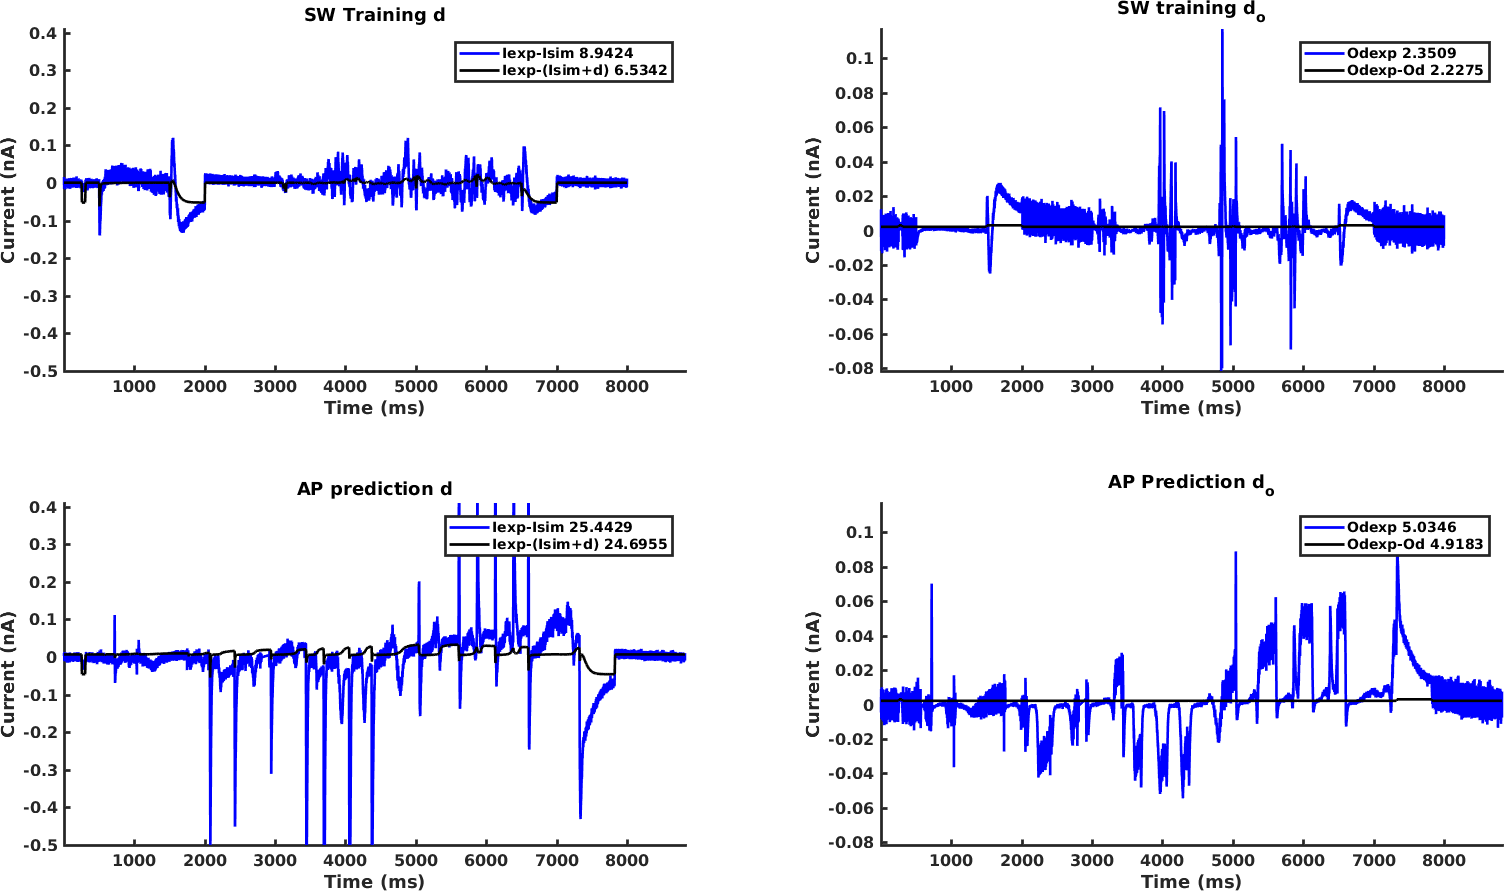
\includegraphics[scale=0.42]{Figures/LASSO_SW_AP_full_discrepancy.png}
\caption{\textbf{Corrected currents using a constructed linear model of discrepancy.} These models of $d$ (left) and $d_o$ (right) in Fig. ~\ref{} have been incorporated into the simulating, giving a revised prediction for the SW and AP protocols. As expected from Fig.~\ref{Fig_LASSO_SW_AP_full_discrepancy}, there is little improvement.}
\label{Fig_LASSO_SW_AP_full_currents}
\end{center}
\end{figure}

Included parameters and their coefficients are shown in Fig.~\ref{Fig_LASSO_SW_AP_coefficients}. The parameters differ considerably between the models for $d$ and $d_o$. Fig.~\ref{Fig_LASSO_SW_AP_lambda} shows the plot of $\lambda$ as a function of MSE. The model with the minimum MSE is indicated by the green line and the model with the largest value of $\lambda$ (hence, the smallest model) within one standard error of the minimum MSE model is shown by the blue line. 

\begin{figure}[t]
\begin{center}
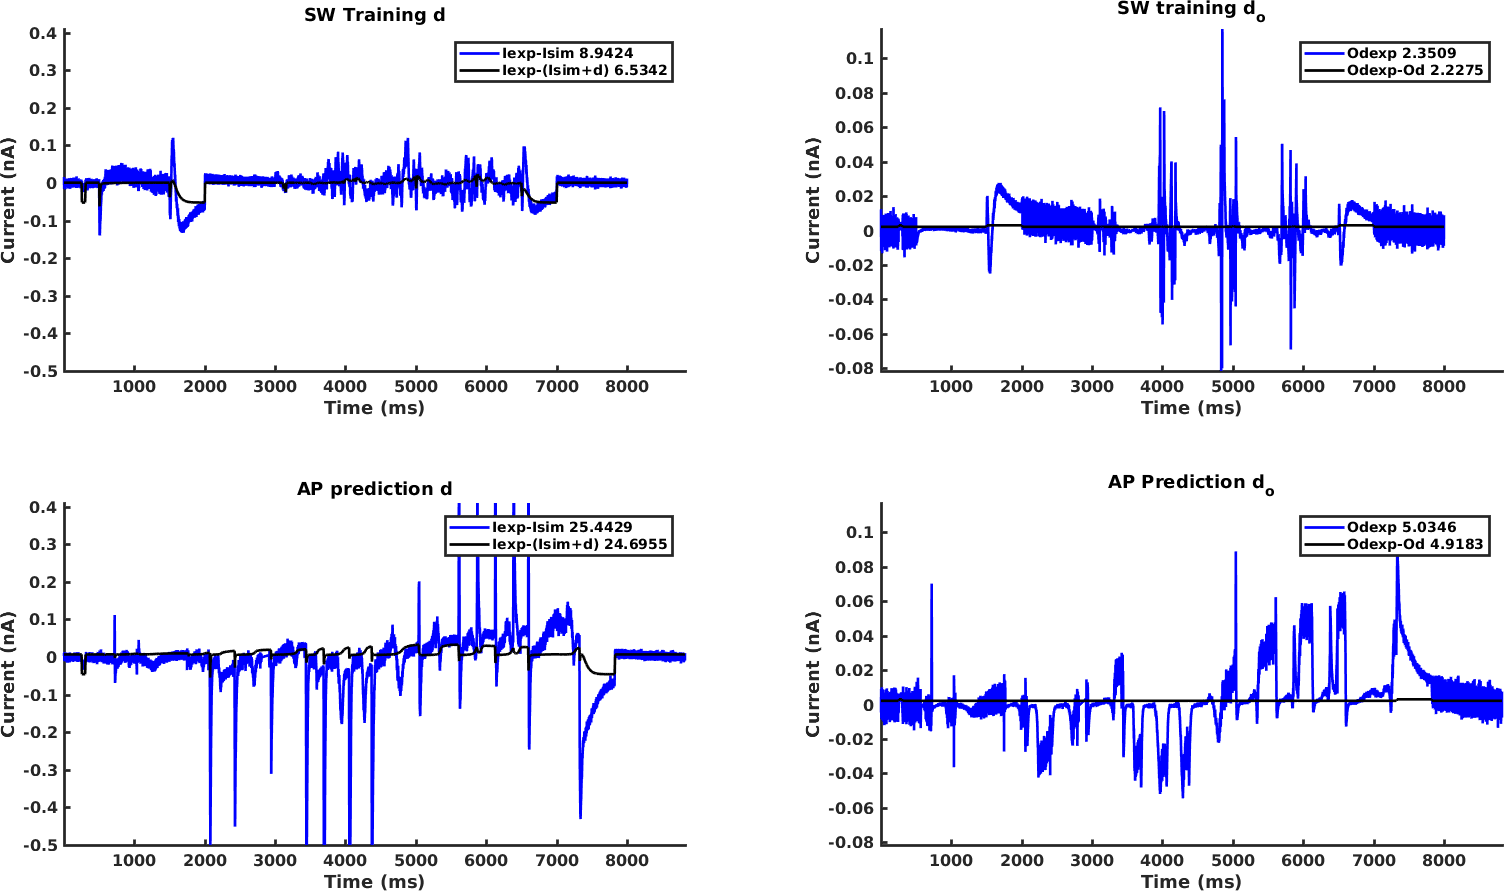
\includegraphics[scale=0.42]{Figures/LASSO_SW_AP_full_discrepancy.png}
\caption{\textbf{Coefficients in the linear model of discrepancy constructed using LASSO.} These models of $d$ (left) and $d_o$ (right) were constructed using LASSO on the entire SW trace (top), starting with all linearly independent predictors. The improvement of the training trace (top) is poor and the resulting models fail to predict the discrepancy in the AP trace (bottom). The root mean square errors between the simulated and predicted traces are shown in the legends. } 
\label{Fig_LASSO_SW_AP_coefficients}
\end{center}
\end{figure}

\begin{figure}[hbt]
\begin{center}
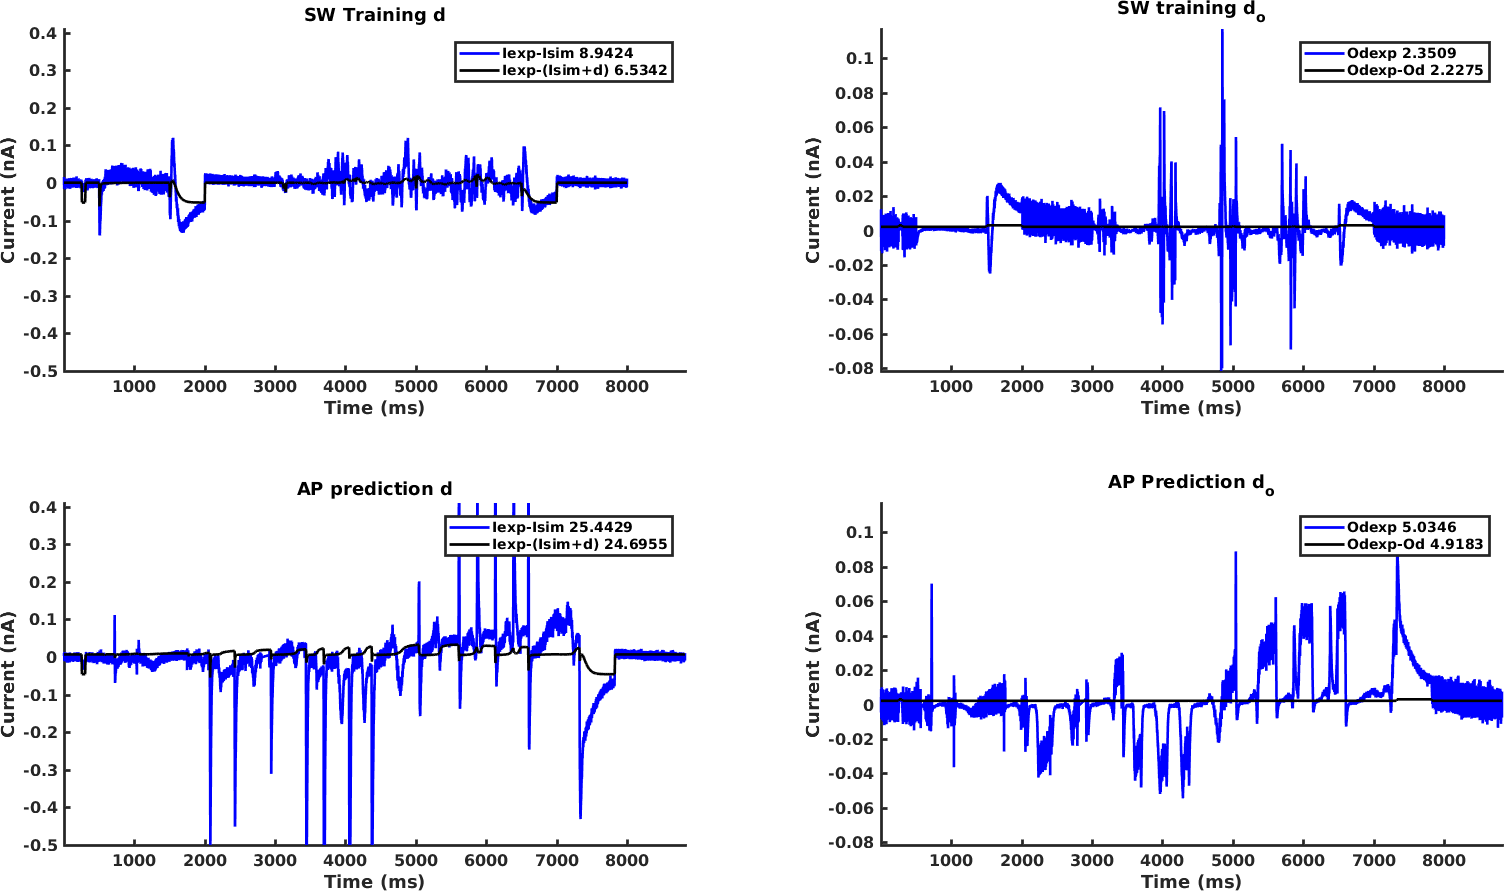
\includegraphics[scale=0.42]{Figures/LASSO_SW_AP_full_discrepancy.png}
\caption{\textbf{Corrected currents using a constructed linear model of discrepancy.} These models of $d$ (left) and $d_o$ (right) in Fig. ~\ref{} have been incorporated into the simulating, giving a revised prediction for the SW and AP protocols. As expected from Fig.~\ref{Fig_LASSO_SW_AP_full_discrepancy}, there is little improvement.}
\label{Fig_LASSO_SW_AP_lambda}
\end{center}
\end{figure}

Based on the failure of the `naive' LASSO method in this case, we also addressed the following hypotheses:
\begin{itemize}
\item the LASSO method might be biased by the large errors that occur in the deactivation steps, and so fail to fit the more subtle errors in the main part of the trace.
\item Because the fit to the SW protocol is `optimal' and  extremely good, there may simply not be enough information in the discrepancy of the sine wave protocol to train a model.
\end{itemize}

To address the first hypothesis, we tried fitting a model to only the sine wave generated part of the SW protocol, and omit the activation and deactivation steps on either end (see Fig.~\ref{Fig_Protocols}). These were then used to predict only the section of the AP protocol containing the action potentials. To address the second hypothesis, we instead trained the models using alternative protocols (OSW, EP, MWDD) that were recorded during the course of the sine wave protocol study. Results for each of these approaches are shown in Fig.~\ref{}-\ref{}. In each case, the linear model of discrepancy only provides marginal gains in the training data, and either fails to improve the discrepancy in the prediction (AP) trace or makes it worse. In general, across all sets of results, the discrepancy in the open probability, $d_o$, appears to be both harder to predict and lead to more over-fitting than the standard definition, $d$.

\subsection{Predicting Discrepancy Using StepwiseLM}\label{SubSec_StepwiseLM_Discrepancy}
\subsubsection{The Method}
Stepwise Linear Model (StepwiseLM) is a Matlab method ...
\subsubsection{Results}

\subsection{Artificial Data}

\subsection{Conclusions}


\section{Parameter Fits Using Alternate Protocols}

\section{Discrepancy Between Alternate Model Structures}

\section{Future Work}

\section{Acknowledgements}
We would like to thank Dr.~Simon Preston and Dr.~Theo Kypraios (University of Nottingham) for useful discussions on LASSO and K-fold cross validation\; Dr.~Kylie Beattie (GlaxoSmithKline) for help with data processing and implementation of alternate pacing protocols\; and Dr.~Michael Clerx and Dr.~Sanmitra Ghosh (University of Oxford) for useful discussions on Hodgkin-Huxley models and model discrepancy.

\end{document}
